\documentclass[10pt]{article}
\usepackage[letterpaper,margin=0.9in]{geometry}
\usepackage{amsmath,mathtools,booktabs,graphicx,float}

\setlength{\parindent}{0pt}\setlength{\parskip}{4pt}
\newcommand{\cl}[1]{\mathsf{#1}}
\newcommand{\col}[3]{\par\smallskip\textbf{#1}\ \ ``#2''. #3}
\allowdisplaybreaks
\AtBeginDocument{\setlength{\abovedisplayskip}{2pt}\setlength{\belowdisplayskip}{3pt}\setlength{\abovedisplayshortskip}{0pt}\setlength{\belowdisplayshortskip}{3pt}}
\makeatletter\renewcommand\section{\@startsection{section}{1}{0pt}{-8pt}{3pt}{\normalfont\large\bfseries}}\makeatother
\begin{document}
{\centering\large\textbf{Chris's spreadsheet model: column definitions and comparison with $A_F(\ell)$}\par\normalsize 25 September 2026\par}

\section{Workbook}
File: \texttt{b3737b04\ldots.xlsx} (copied to \texttt{chris\_model.xlsx}). The per-angle model is on the tab
\emph{density w rotation} and its three copies; all four tabs have identical row formulas and differ only in
parameter cells (Table~\ref{tab:tabs}). Numbers below are from \emph{Copy of Copy of Copy of density}, the tab
recorded as the working set in our 18~Sep notes. Rows 66--426 hold $\theta=0,1,\dots,360^\circ$. The final
column is \textbf{BH}, ``Model A/A\_all''; the sheet's chart ``a and migkas'' plots BH against the Migkas column BI.

The other two workbooks are not this model: \texttt{9033\ldots.xlsx} is our own calculator
(\texttt{A\_vs\_angle\_calc.xlsx}), and \texttt{37301\ldots.xlsx} is an earlier point-mass version
(the \emph{point} tab here; no A column, force $\propto 1/r$).

Geometry, as the formulas define it: plane $(x,y)$, centre of expansion (CoE) at the origin, Earth at $(D,0)$.
The source P lies on a circle of radius $R$ about Earth, at viewing angle $\theta$ measured from $+x$;
$\theta=0$ looks directly away from the CoE and $\theta=180^\circ$ looks at it.

\section{Parameter cells}
Column letters in sans serif ($\cl{C}$, $\cl{L}$, \dots) are sheet columns in the same row; italic symbols are parameter cells.

\begin{table}[H]\centering\small
\begin{tabular}{@{}llll@{}}\toprule
Cell & Label (his) & Formula & Value \\\midrule
C23 & -- & input & 5 \quad($=D/R$)\\
D23 & -- & input & 0.18 \quad($=L/D$)\\
B25 & $k$ ``1/s, Taylor Sedov Hubble constant'' & input & $2.18\times10^{-18}$\\
B26 & $G$ ``N(km/kg)$^2$'' & input & $6.67\times10^{-17}$\\
B27 & $M$ ``kg'' & $=\mathrm{D27}\cdot\mathrm{E27}\cdot10^{13}$, D27 $=10^{53}$, E27 $=444$ & $4.44\times10^{68}$\\
B28 & $D$ ``km, Earth to coe'' & $=\mathrm{B29}\cdot\mathrm{C23}$ & $6.5\times10^{23}$\\
B29 & $R$ ``km, Earth to P'' & input & $1.3\times10^{23}$\\
B30 & $L$ ``km, density distribution'' & $=\mathrm{B28}\cdot\mathrm{D23}$ & $1.17\times10^{23}$\\
B32 & $V_o$ ``observer velocity, all x'' & $=kD$ & $1.417\times10^{6}$\\
B33 & $dt$ & input & 1\\
B34 & $A_{x,\rm obs}$ ``observer acceleration, all x'' & $=-GM/D^2$ & $-7.009\times10^{4}$\\
B36 & $v^*$ & $=Rk$ & $2.834\times10^{5}$\\
B55 & $f_D$ ``fraction up to o'' & $=1-e^{-D/L}(1+D/L+D^2/2L^2)$ & 0.91500\\
B56 & $M_{\rm tot}$ ``total mass'' & $=M/f_D$ & $4.852\times10^{68}$\\
E39 & -- & input (subtracted from Migkas $B$) & 0.09\\
BA57 & amplitude, A rotation & input & $-0.06$\\
BA58 & $\omega$ & $=2\pi/360$ & 0.0174533\\
BA59 & phase $\phi$ (rad) & input & 0.35\\
BE57--59 & B rotation & $=-\mathrm{BA57}$, BA58, BA59 & $+0.06$, $\omega$, 0.35\\\bottomrule
\end{tabular}\end{table}
Cells not used by any row formula: B7--B10 ($c=100$, $v/c$, $\sqrt{1-v^2/c^2}$, which shows \texttt{\#NUM!}),
unlabelled B12--B18, B23 ($L=0.5$), D27--E28, D29 $=(D/R)^3$, B54, C54, D54.

\section{Columns, in sheet order}
Dependencies are listed after each header. Row 66 differs from the other rows only in column G (noted there).

\col{A}{degrees}{Viewing angle $\theta$ from Earth. Input.}
\begin{equation}\cl{A}=\theta\end{equation}
\col{B}{radians}{From A.}
\begin{equation}\cl{B}=\pi\,\cl{A}/180\end{equation}
\col{C}{px}{$x$ of P. From B; $D$, $R$.}
\begin{equation}\cl{C}=D+R\cos\cl{B}\end{equation}
\col{D}{py}{$y$ of P. From B; $R$.}
\begin{equation}\cl{D}=R\sin\cl{B}\end{equation}
\col{E}{D}{Distance of P from the CoE. From C, D.}
\begin{equation}\cl{E}=\sqrt{\cl{C}^2+\cl{D}^2}\end{equation}
\col{F}{V=kD}{Sedov--Taylor speed of P about the CoE. From E; $k$.}
\begin{equation}\cl{F}=k\,\cl{E}\end{equation}
\col{G}{theta}{Polar angle of P seen from the CoE. From C, D. Row 66 adds \texttt{RADIANS(B58)}; B58 is empty, so it adds 0.}
\begin{equation}\cl{G}=\arctan(\cl{D}/\cl{C})\end{equation}
\col{H}{Vx}{From F, G.}
\begin{equation}\cl{H}=\cl{F}\cos\cl{G}\end{equation}
\col{I}{Vy}{From F, G.}
\begin{equation}\cl{I}=\cl{F}\sin\cl{G}\end{equation}
\col{J}{dVx}{Velocity of P relative to Earth, $x$. From H; $V_o$.}
\begin{equation}\cl{J}=\cl{H}-V_o\end{equation}
\col{K}{dVy}{Same, $y$ (Earth has no $y$ velocity). From I.}
\begin{equation}\cl{K}=\cl{I}\end{equation}
\col{L}{recession v*}{Relative speed without gravity. From J, K. Algebraically $\cl{J}=kR\cos\theta$ and $\cl{K}=kR\sin\theta$, so $\cl{L}=kR=v^*$ in every row.}
\begin{equation}\cl{L}=\sqrt{\cl{J}^2+\cl{K}^2}\end{equation}
\col{AO}{mass up to P}{Mass inside radius $\cl{E}$ for $\rho\propto e^{-r/L}$, scaled so that the mass inside $D$ equals $M$. From E; $L$, $M_{\rm tot}$. (It sits in column AO, but N uses it.)}
\begin{equation}\cl{AO}=\Bigl[1-e^{-\cl{E}/L}\Bigl(1+\frac{\cl{E}}{L}+\frac{\cl{E}^2}{2L^2}\Bigr)\Bigr]M_{\rm tot}\end{equation}
\col{N}{A}{Gravitational acceleration of P toward the CoE. From E, AO; $G$.}
\begin{equation}\cl{N}=-G\,\cl{AO}/\cl{E}^2\end{equation}
\col{O}{Ax}{From N, G.}
\begin{equation}\cl{O}=\cl{N}\cos\cl{G}\end{equation}
\col{P}{Ay}{From N, G.}
\begin{equation}\cl{P}=\cl{N}\sin\cl{G}\end{equation}
\col{Q}{dAx}{Acceleration of P relative to Earth, $x$. From O; $A_{x,\rm obs}$.}
\begin{equation}\cl{Q}=\cl{O}-A_{x,\rm obs}\end{equation}
\col{R}{dAy}{Same, $y$. From P.}
\begin{equation}\cl{R}=\cl{P}\end{equation}
\col{S}{dVx*}{Relative velocity after one step of relative acceleration, $x$. From J, Q; $dt$.}
\begin{equation}\cl{S}=\cl{J}+\cl{Q}\,dt\end{equation}
\col{T}{dVy*}{Same, $y$. From K, R; $dt$. The terms are in the opposite order to S (see item 1 in Sec.~6).}
\begin{equation}\cl{T}=\cl{R}+\cl{K}\,dt\end{equation}
\col{U}{recession v}{Relative speed with gravity. From S, T.}
\begin{equation}\cl{U}=\sqrt{\cl{S}^2+\cl{T}^2}\end{equation}
\col{X}{angle v}{Direction of $(\cl{S},\cl{T})$; a diagnostic, not used downstream. Excel \texttt{ATAN2(S,T)}.}
\begin{equation}\cl{X}=\operatorname{atan2}(\cl{T},\cl{S})\end{equation}
\col{Y}{angle a}{Direction of the acceleration of P; a diagnostic. From O, P.}
\begin{equation}\cl{Y}=\arctan(\cl{P}/\cl{O})\end{equation}
\col{AB, AC}{recession v*, (recession v)}{Plot copies. From L, U.}
\begin{equation}\cl{AB}=\cl{L},\qquad \cl{AC}=\cl{U}\end{equation}
\col{AF}{(recession v); plotted as ``A/A\_all Model''}{Ratio of speed with gravity to speed without gravity. From U, AB.}
\begin{equation}\cl{AF}=\cl{U}/\cl{AB}\end{equation}
\col{BA}{model}{Sine ``rotation'' term in the sheet angle $\theta$; $\omega\theta$ is in radians. From A (through AR $=$ AJ $=$ AA $=$ A); BA57--59.}
\begin{equation}\cl{BA}=\mathrm{BA57}\,\sin(\omega\,\theta+\phi)\end{equation}
\col{BH}{Model A/A\_all}{\textbf{Final A column.} From AF, BA.}
\begin{equation}\cl{BH}=(1-\cl{BA})\,\cl{AF}\end{equation}
The B branch: \textbf{AN} ``mass up to p x'' $=\cl{AO}/M$; \textbf{BE} $=\mathrm{BE57}\sin(\omega\theta+\phi)$; \textbf{BL} ``Model B/B\_all'' $=(1-\cl{BE})\,\cl{AN}$.

Written out, with $dt$ kept:
\begin{equation}
\cl{BH}(\theta)=\bigl[1-a_A\sin(\omega\theta+\phi)\bigr]\,
\frac{\bigl|\,kR\,\hat{\mathbf n}(\theta)+dt\,[\mathbf g(\mathbf r_P)-\mathbf g(D\hat{\mathbf x})]\,\bigr|}{kR},
\qquad \mathbf g(\mathbf r)=-\frac{G\,m(r)}{r^2}\hat{\mathbf r},
\end{equation}
where $a_A=\mathrm{BA57}$ and $m(r)=\cl{AO}$. The $y$ part matches this only because $dt=1$ (item 1).

\paragraph{Comparison columns (no effect on BH).}
AD, AL: angle, copied. AG $=$ \texttt{VLOOKUP(AD$_{n+10}$, migkas!E:H, 3, TRUE)} gives Migkas $A$; AM is the same lookup for Migkas $B$, minus E39.
AE $=$ AG; BI $=$ AG; BM $=$ AM. AH $=|\cl{AF}-\cl{AG}|$, AI $=(\cl{AF}-\cl{AG})/\cl{AF}$, AP $=|\cl{AM}-\cl{AN}|$, AQ $=(\cl{AN}-\cl{AM})/\cl{AN}$; AZ $=$ AI and BD $=$ AQ.
BJ $=(\cl{BH}-\cl{BI})/\cl{BH}$, BN $=(\cl{BL}-\cl{BM})/\cl{BL}$. AK $=10^{\cl{AF}}/2$. AS $=$ AF shifted by $180^\circ$.
AV--AY are helper columns. Summary cells: AF49, AM49, BH56 and BL56 are \texttt{LINEST} fits; BH58 is the $R^2$ of BI on BH (0.7389); D3 $=$ BH58/AF51 ``R2w/R2wo''.

\section{Recomputation check}
\texttt{recompute\_columns.py} implements Eqs.~(1)--(27) literally and compares them with the values cached in the file.
Model columns B--BL agree to a maximum relative difference of $4\times10^{-6}$ (primary tab; $\le 2\times10^{-5}$ on all four tabs).
The residual differences come from the file storing about 7 significant figures. For BH alone the difference is $1.5\times10^{-7}$.
The lookup columns AG and AM agree except on 7 and 8 rows. On those rows $\theta+10$ is a multiple of 8, so the lookup key falls
exactly on a node of the $360/315$ grid and the sheet's rounding decides which side is taken. Using the cached AG, the sheet's own $R^2$ is reproduced (0.73894 vs BH58 $=$ 0.73894).

\section{Comparison with $A_F(\ell)$ and the Migkas points}
$A_F(\ell)=0.9965+0.0296\cos\ell+0.0434\sin\ell+0.0636\cos2\ell+0.0366\sin2\ell-0.0299\cos3\ell-0.0114\sin3\ell$.
Two angle mappings are used. (i) $\theta=\ell$. (ii) The sheet's lookup mapping, which pairs row $\theta$ with Migkas
$\ell=45+\lfloor\tfrac78(\theta+10)\rfloor$ (item 4). Here $R^2=1-\sum(y-\cl{BH})^2/\sum(y-\bar y)^2$ has no refit;
$r^2$ is the squared correlation, which is what \texttt{LINEST} reports.

\begin{table}[H]\centering\small
\begin{tabular}{@{}lcccc@{}}\toprule
Comparison (primary tab) & $N$ & RMS & $R^2$ & $r^2$\\\midrule
BH vs $A_F$, $\theta=\ell$, $0$--$359^\circ$ & 360 & 0.0376 & 0.691 & 0.779\\
AF (no sine term) vs $A_F$, $\theta=\ell$ & 360 & 0.0522 & 0.406 & --\\
BH vs 71 Migkas points, $\theta=\ell$ & 71 & 0.0429 & 0.632 & 0.712\\
BH vs Migkas points, sheet mapping (ii) & 62 & 0.0576 & 0.259 & 0.532\\
$A_F$ vs 71 Migkas points & 71 & 0.0206 & 0.915 & --\\
Sheet's own BI vs BH (cell BH58) & 361 & -- & -- & 0.739\\\bottomrule
\end{tabular}\end{table}

\begin{table}[H]\centering\small
\setlength{\tabcolsep}{4pt}\begin{tabular}{@{}lrrrrrrrrrrrr@{}}\toprule
$\theta=\ell$ ($^\circ$) & 0 & 30 & 60 & 90 & 120 & 150 & 180 & 210 & 240 & 270 & 300 & 330\\\midrule
$\cl{BH}-A_F$ & .029 & $-.002$ & $-.024$ & .019 & .082 & .080 & .016 & $-.022$ & $-.001$ & .021 & .017 & .023\\\bottomrule
\end{tabular}\end{table}

The largest residual is $+0.092$ at $134^\circ$. There $A_F$ and the data dip to $\approx0.89$ near $125^\circ$, while BH stays near 1.0.
The mean of BH over $\theta$ is 1.0164, against 0.9965 for $A_F$.
Elsewhere BH follows $A_F$ to within about 0.03: the maximum near $20^\circ$, the second maximum near $180^\circ$, and the minimum near $260^\circ$.

\begin{figure}[H]\centering
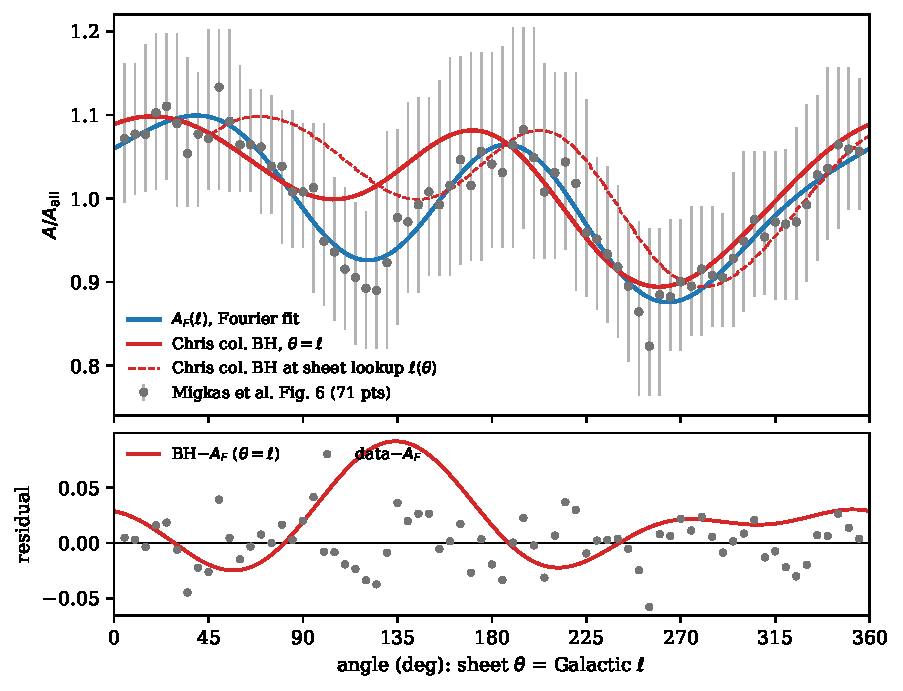
\includegraphics[width=0.74\linewidth]{A_compare.pdf}
\caption{Top: BH (primary tab) at $\theta=\ell$ (solid) and at the sheet's lookup mapping (dashed), $A_F$, and the Migkas points. Bottom: BH$-A_F$ and data$-A_F$.}
\end{figure}

\begin{table}[H]\centering\small
\setlength{\tabcolsep}{4pt}\begin{tabular}{@{}lcccccccc@{}}\toprule
Tab & $D/R$ & $L/D$ & $GM\,dt/D^2kR$ & BA57 & $\phi$ & BH58 & RMS vs $A_F$ & $R^2$ vs data\\\midrule
density w rotation & 3.33 & 0.150 & 0.167 & $-0.055$ & 0.15 & 0.686 & 0.0436 & 0.531\\
Copy of density w rot. & 9.00 & 0.250 & 0.414 & $-0.06$ & 0 & 0.594 & 0.0416 & 0.566\\
Copy of Copy of \ldots & 6.10 & 0.199 & 0.331 & $-0.06$ & 0.40 & 0.745 & 0.0369 & 0.644\\
Copy of Copy of Copy (primary) & 5.00 & 0.180 & 0.247 & $-0.06$ & 0.35 & 0.739 & 0.0376 & 0.632\\\bottomrule
\end{tabular}
\caption{The four working tabs ($R^2$ vs data: 71 points, $\theta=\ell$). The fifth copy replaces S and $V_o$ with escape-speed expressions; its cached BH58 is $8\times10^{-4}$ and D3 shows \texttt{\#DIV/0!}, so it is omitted.}\label{tab:tabs}
\end{table}

\section{Points for Chris}
\begin{enumerate}\setlength{\itemsep}{1pt}
\item \textbf{T} $=\cl{R}+\cl{K}\,dt$, whereas \textbf{S} $=\cl{J}+\cl{Q}\,dt$. The form parallel to S is $\cl{K}+\cl{R}\,dt$. With $dt=1$ the two give the same number, but only then. Which is intended?
\item $dt=1$ multiplies an acceleration that is then added to a velocity. The size of the anisotropy is set by the ratio $GM\,dt/(D^2kR)$, which is 0.247 here and depends on the time unit. What sets $dt$?
\item $G=6.67\times10^{-17}$ is labelled N(km/kg)$^2$. In km and s, SI $G$ is $6.67\times10^{-20}$ km$^3$\,kg$^{-1}$\,s$^{-2}$. Only the product $GM$ enters, so this is equivalent to a 1000$\times$ larger $M$.
\item Migkas lookup: AG in row $\theta$ uses key $\theta+10$ on \texttt{migkas!E}, a uniform grid of step $360/315$ that indexes $\ell=46\ldots360$. The model at $\theta$ is therefore compared with $\ell=45+\lfloor\frac78(\theta+10)\rfloor$, which is a $10^\circ$ offset plus a 7/8 stretch; $\ell<46^\circ$ is never used. Is that intended, or should $\theta=\ell$? Against the Migkas points, $R^2$ is 0.63 with $\theta=\ell$ and 0.26 with the sheet mapping.
\item BA is a sine in $\theta$ with a set amplitude and phase, applied after the geometry. Is it meant as a physical term (rotation of the CoE axis), or as a fit factor?
\item Header ``D'' on column E is the CoE--P distance; the \emph{terms} tab calls it ``distance from earth to coe''.
\item Column L equals $kR$ in every row, so AF $=$ U$/(kR)$. Please confirm this normalisation is the intended $A_{\rm all}$.
\item Which tab is current? The formulas are the same on all four; the parameters and $R^2$ differ (Table~\ref{tab:tabs}).
\end{enumerate}

\sloppy\footnotesize Files: \texttt{papers/spreadsheet\_model/}\{\texttt{columns.tex}, \texttt{recompute\_columns.py}, \texttt{recompute\_results.json}, \texttt{primary\_columns.csv}, \texttt{make\_figure.py}, \texttt{A\_compare.pdf/png}, \texttt{chris\_model.xlsx}\}.
\end{document}
